
\documentclass[11pt,letterpaper]{article}

% Packages:
\usepackage{geometry}
\usepackage{amsmath,amssymb}
\usepackage{enumerate}
\usepackage{listing}
\usepackage{lipsum}
\usepackage{graphicx}
\usepackage{hyperref}
\usepackage{booktabs}
\usepackage{pdfpages}
 
% Page style:
\geometry{top=2cm, bottom=2cm, left=2.5cm, right=2.5cm}
\linespread{1.3} % 1.3 for one-and-a-half spacing, 1.6 for double spacing


% Fields:
\newcommand{\assignmenttitle}{Midterm}
\newcommand{\course}{MATH 423 Applied Regression}
\newcommand{\studentid}{Su Goh \\ 260780918}


\begin{document}
	
	\noindent
	\large \textbf{\course { -- } \assignmenttitle} \\
	\studentid \\
	\noindent\rule{\textwidth}{0.4pt}
	
	\section*{Question 1}
		\paragraph*{1.1} The t-value is 1.03881.
		\begin{align*}
		T_0 &= \frac{\hat{\beta_0}}{ese(\hat{\beta_0)}} \\ 
			&= \frac{0.13088}{0.12599} \\ 
			&= 1.03881
		\end{align*}
		
		\paragraph*{1.1} The hypothesis as follows: 
		\begin{align*}
			H_0 : \beta_1 = 0 \\
			H_1: \beta_1 \neq 0
		\end{align*}
		The p-value represents the probability that we obtain the observed t-statistic under the assumption that \(H_0\) is true. Reading off from the table, p-value = \(Pr(>|t|) = 7.55e^{-12}\), which is extremely small. At \(\alpha = 0.05\), we can reject the null hypothesis and conclude that \(X_1\) has some influence on the dependent variable in our model. 
		
		\paragraph*{1.3} For the simple linear regression model, degrees of freedom is given by n-2, as there are 2 coefficients. \(n = 25 \implies n-2 = 23\). It has 23 degrees of freedom. 
		
		\paragraph*{1.4} From the table, residual standard error \(\equiv \hat{\sigma} = 0.2361\). Thus \(\hat{\sigma}^2 = 0.2361^2 = 0.05574\).
		\begin{align*}
			\hat{\sigma} &= \sqrt{\frac{SS_{Res}}{df_{Res}}} \\
			0.2361^2 &= \frac{SS_{Res}}{23} \\ 
			\implies SS_{Res} &= 0.05574 \cdot 23 \\
				&= 1.28209	
		\end{align*}
	
		\paragraph*{1.5} 
		\begin{align*}
			ese(\hat{\beta_1}) &= \sqrt{\frac{\hat{\sigma}^2}{S_{xx}}} \\
			0.01905^2 &= \frac{0.05574}{S_{xx}} \\
			\implies S_{xx} &= 153.595
		\end{align*}
		 
		\paragraph*{1.6} I assume that all the SLR assumptions hold for this model. Specifically, that the errors are independent and have mean 0. If the assumptions hold, then we also know that the estimators are unbiased, i.e. \(\mathbb{E}(\beta_j) = \hat{\beta_j} , \forall j=0,1\).
		\begin{align*}
			\mathbb{E}(Y|X_1 = 0) &= \mathbb{E}(\beta_0 + \beta_1 X_1 + \epsilon | X_1 = 0) \\
				&= \mathbb{E}(\beta_0) + \mathbb{E}(\beta_1X_1 | X_1 = 0) + \mathbb{E}(\epsilon) \\
				&= \hat{\beta_0} + 0 + 0 \\ 
				&= \hat{\beta_0} \\ 
				&= 0.13088
		\end{align*}	 
		
		\paragraph*{1.7} The confidence interval is 95\%CI(\(\beta_1\)) = \([0.2017426, 0.2805551]\). We can interpret it as such: if we run the experiment 100 times, 95 of the confidence intervals constructed from the sample's \(\hat{\beta_1}\) will contain the true value \(\beta_1\). The estimate for the coefficient of \(X_1\) is statistically significant at the 95\% confidence level, and from the above CI, we can conclude that \(X_1\), velocity, has a small positive effect on \(Y\), electricity output. Holding all else constant, an increase in velocity by 1 unit will contribute to an increase in electricity output by 0.20 to 0.28 units. 		
		
		\paragraph*{1.8} We can construct confidence intervals with the following formula:
		\begin{equation*}
			CI(\beta_0) = [\hat{\beta_0} - k \cdot ese(\hat{\beta_0}), \hat{\beta_0} + k \cdot ese(\hat{\beta_0})] \\ 
		\end{equation*}
		k is given as 2.068658 and we have the following values: \(\hat{\beta_0} = 0.13088, ese(\hat{\beta_0}) = 0.12599\).
		Hence, we can compute the CI:
		\begin{align*}
			CI(\beta_0) &= [0.13088 - 2.068658 \cdot 0.12599, 0.13088 + 2.068658 \cdot 0.12599] \\ 
				&= [-0.12975, 0.39151]
		\end{align*}
	
	\newpage
	
	\section*{Question 2 - Data Analysis}
	
	\paragraph*{Research Problem}
	We are interested in identifying if the height of abalones can be used to predict their ages. Generally, the age of abalones was identified by counting the number of rings on the abalone's shell. However, there are other variables that affect the growth of the abalone's shell, such as the availability of food, which can vary significantly across different habitats. Can other physical characteristics of the abalone, specifically its height, affect its rings too? The following model will investigate the relationship:
	\[\text{rings}_i = \beta_0 + \beta_1 \cdot \text{height}_i + \epsilon_i\]
	\begin{itemize}
		\item \textit{rings}: the dependent variable, the number of rings in the abalone's shell, which is a proxy for  the age of the abalone.
		\item \textit{height}: the independent variable, the height of the abalone.
	\end{itemize}

	It is hypothesized that height and the number of rings are positively related: a taller height implies that the abalone is older.
	
	\paragraph*{Data Description}
	The dataset contains 4177 observations and has 2 variables, rings and height. Height is measured in mm.\footnote{\url{https://archive.ics.uci.edu/ml/datasets/abalone}}
	
	The distribution of the number of rings the abalones in the dataset have are depicted in a histogram (Figure \ref{fig:rings}). The data is skewed to the right: most of the data points are clustered around the mean (in red) and on the left of it, but there is a long right tail. The number of abalones' rings range from 1 to 29. The average number of rings is 9.934 and the median is 9. The variance of the number of rings is 10.3952. 

	\begin{figure}
		\centering
		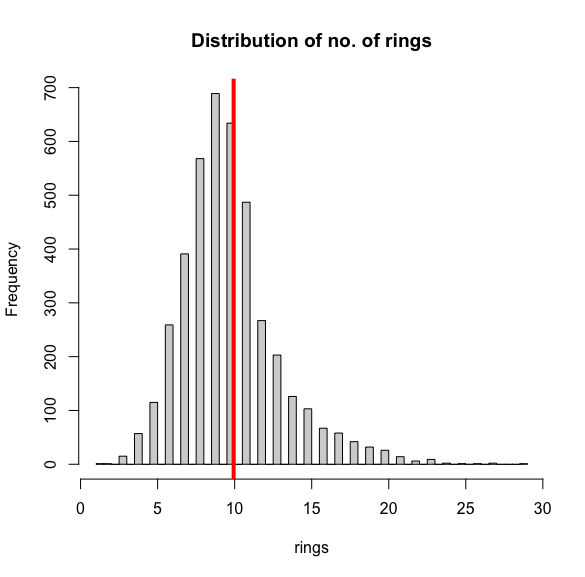
\includegraphics[height=0.4\textheight]{2-rings}
		\caption{Distribution of abalone rings}
		\label{fig:rings}
	\end{figure}

	The distribution of the abalone height is plotted in a histogram (Figure \ref{fig:height}). The histogram is clustered closely around the mean, however there are some outlying values far in the right tail, which contributes to the variance of the data points. The heights range from 0 mm to 1.13 mm. The mean of the data is 0.14 mm and the median is 0.1395 mm. The variance is 0.001749503. 
	
	\begin{figure}
		\centering
		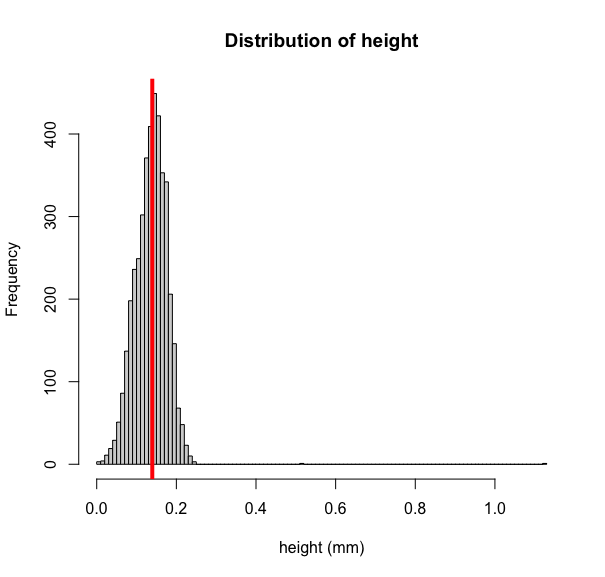
\includegraphics[height=0.4\textheight]{2-height}
		\caption{Distribution of abalone heights}
		\label{fig:height}
	\end{figure}

	\paragraph*{Scatter plot, Estimation \& Model Fit}
	
	\begin{figure}
		\centering
		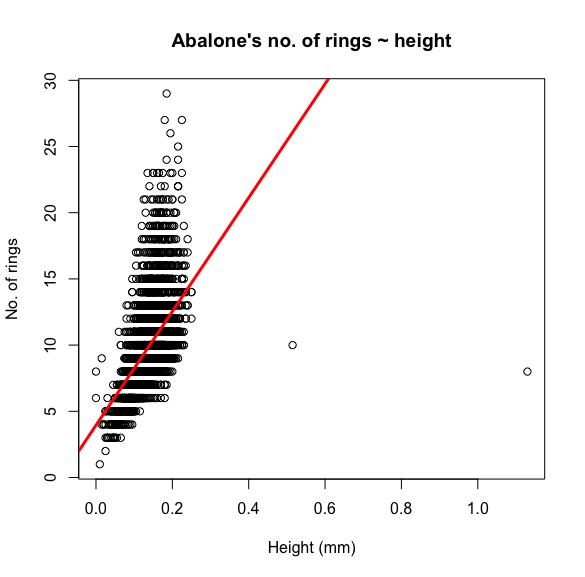
\includegraphics[height=0.4\textheight]{2-scatterplot}
		\caption{Scatter plot of abalone data.}
		\label{fig:scatterplot}
	\end{figure}

	The scatter plot of the data (Figure \ref{fig:scatterplot}) suggests that there is no linear relationship between the number of rings and the abalone's height. There is a large cluster of data points for observations of height from 0 to 0.2mm that appear almost vertical and leaning slightly to the right. There are also 2 points far on the right of this large cluster. They appear to be outliers, as they are so far from the rest of the data.  
	
	A simple linear regression using least squares is carried out on the data, regressing the number of rings on the abalone's height. The results are in Table \ref{tab:ols}. The model tells us that height is a statistically significant predictor for the number of rings, and a 1mm increase in height will lead to an increase in the number of rings by 42.97. 
	
	\begin{table*}
		\caption{Results of the regression of the number of rings on the abalone's height.}
		\centering
		\begin{tabular}{ccccc}
			\midrule
			~& Estimate & std. error & $t$ & $Pr(>|t|)$\\
			\midrule
			(Intercept) & 3.9385 & 0.1443 & 27.30 & \textless2e-16$^{***}$\\
			Height & 42.9714 & 0.9904 & 43.39 & \textless2e-16$^{***}$\\
			\midrule
		\end{tabular}
		\label{tab:ols}
	\end{table*}
	
	Next, I plot the fitted regression line from the model on the scatter plot. The fitted regression line (in red) depicts a linear relationship between height and number of rings with a positive slope. It is not a good fit for the data as it does not pass through or come close to many of the data points. The outliers affect the estimated regression line by ``pulling" it towards them, contributing to the slope of the line. 
	
	The data is not linear, which means the assumption of linearity in the simple linear regression does not hold. The regression model also has a residual standard error of 2.677, which is quite high. Hence, I will apply a log transformation to the number of rings and re-fit the model. 
	
	\paragraph*{Log-transformed data}
	As discussed previously, the data does not satisfy the linearity assumption and the simple linear regression model was not a good fit. To solve this, I apply a log-transformation on the number of rings. This helps to make shape of the data closer to that of the normal distribution which has a constant variance, as can be seen in Figure \ref{fig:rings-log}. 
	
	\begin{figure}
		\centering
		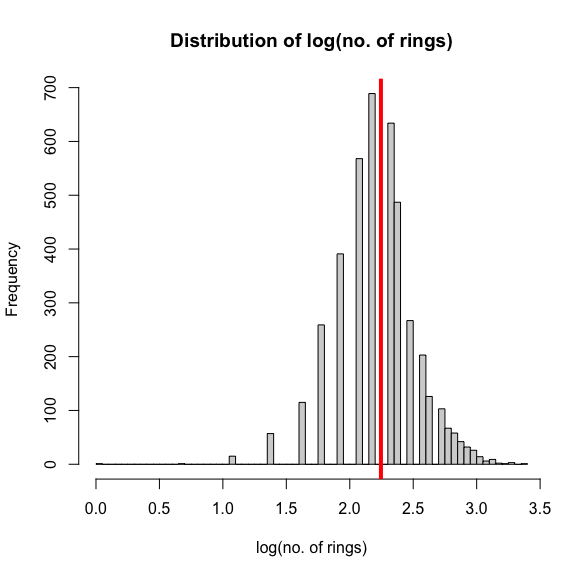
\includegraphics[height=0.4\textheight]{2-rings-log}
		\caption{Histogram of the distribution of log(no. of rings).}
		\label{fig:rings-log}
	\end{figure}

	\begin{figure}
		\centering
		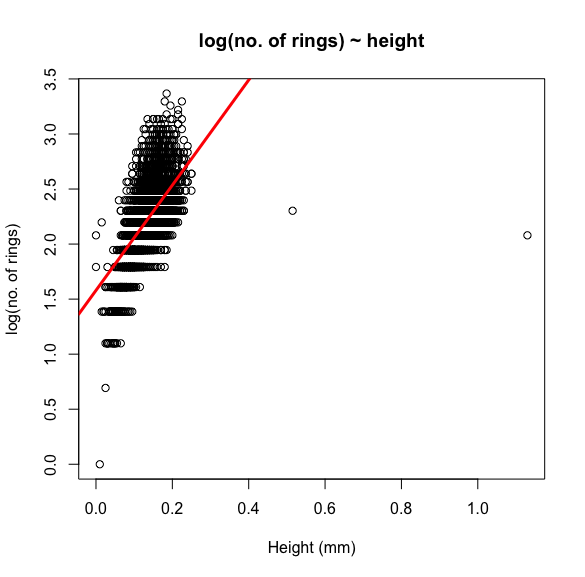
\includegraphics[height=0.4\textheight]{2-log}
		\caption{Scatter plot of log(no. of rings) and height.}
		\label{fig:scatter-log}
	\end{figure}
	
	As can be seen from the scatter plot (Figure \ref{fig:scatter-log}), the cluster of data points is less vertical and appears to be spread in a diagonal rightwards shape, implying a linear relationship. There are still outlying data points, but the fitted regression line (in red) seems to fit the trend of the cluster of data points well. Thus, the log-transformation on the number of rings made it appropriate for us to infer a linear relationship and  apply a simple linear regression to the transformed data.
	
	\paragraph*{Log-transformed data: Results and Interpretation}
	The results of the regression on the transformed data are in Table \ref{tab:log-ols}. The residual error is now 0.2494, which is far less than in the previous model.  
	
	\begin{table*}[hb]
		\caption{Results of the regression of the transformed data.}
		\centering
		\begin{tabular}{ccccc}
			\midrule
			~& Estimate & std. error & $t$ & $Pr(>|t|)$\\
			\midrule
			(Intercept) & 1.57924 & 0.01344 & 117.52 & \textless2e-16$^{***}$\\
			Height & 4.77676 & 0.09226 & 51.77 & \textless2e-16$^{***}$\\
			\midrule
		\end{tabular}
		\label{tab:log-ols}
	\end{table*}
	
	Height has a statistically significant influence on the log of the number of rings. This means that holding all else constant, a 1mm increase in the abalone's height will lead to an expected change by 4.7767 in the log of the number of rings. Note that the model is now $\log(\text{rings}) = \beta_0 + \beta_1 \text{height} + \epsilon$. We take the exponents of both sides to find:
	\begin{align*}
		\exp\{\log(\text{rings})\} &= \exp\{\beta_0 + \beta_1 \text{height} + \epsilon\} \\
		\text{rings} &= \exp\{\beta_0\}\exp\{\beta_1 \text{height}\}\exp\{\epsilon\}
	\end{align*} 
  Hence a 1mm increase in height actually changes the number of rings by a factor of $\exp(4.77676) = 118.7191$. Similarly, when height is 0, the log of the number of rings changes by 1.57924, which means that the number of rings changes by a factor of $\exp(1.57924) = 4.851279$.
  
  At the 95\% level of confidence, the confidence interval for the intercept is $[1.552897, 1.605587]$ and for height is $[4.595882, 4.957639]$. This means that if we were to run this experiment 100 times, 95 of the confidence intervals generated from the estimates of the coefficients would contain the true value. We can thus conclude that height generally has a positive effect on the number of rings.
  
  According to the t-test (results in Table \ref{tab:log-ols}), the coefficients for height is statistically significant at $\alpha=0$, meaning that there is indeed a positive relationship between the two variables. 
  
  From conducting the permutation test, we find that the p-value is 0 (Figure \ref{fig:permute}), meaning we can reject the hypothesis that the coefficient for height is 0. We can conclude that height has a positive relationship with the number of rings, which is in line with the conclusion from the original t-test.
  
	\begin{figure}[h]
	  	\centering
	  	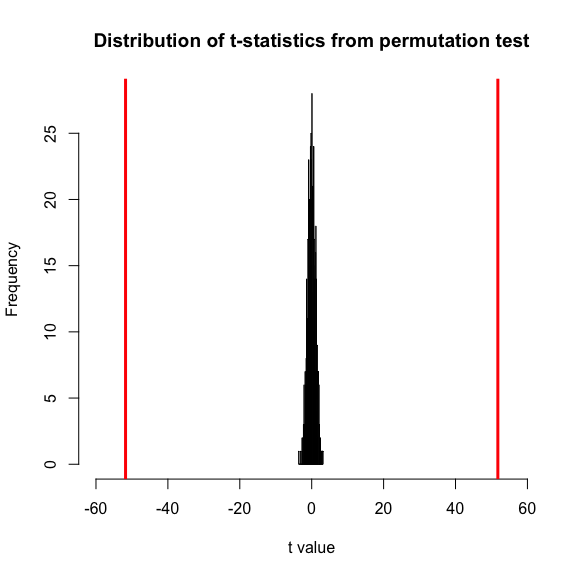
\includegraphics[height=0.4\textheight]{2-permutation}
	  	\caption{Histogram of t-statistics from 1000 permutations. The red lines represent the original t-statistic.}
	  	\label{fig:permute}
  	\end{figure}
  
  \paragraph*{Prediction}
  When height = 0.132, the log of the number of rings is 2.209775. 
  
  \paragraph*{Conclusion}
  We first noted that the relationship between the height of the abalone and the number of rings it has, a proxy for its age, is not linear. After applying a log transformation to the number of rings, we found that while the relationship between the two variables is not linear, it does exist, and it is positive. The results corroborate the hypothesis that the height of an abalone positively varies with its age, i.e. an older abalone is taller. I note that for the model on transformed data, the $R^2 = 0.391$, while the t-test tell us that height is statistically significant. This implies that height is a useful predictor, but not sufficient. To make the predictive power of the model stronger, other physical features of the abalone should be added. This would help the researchers to identify the factors that come together to affect the number of rings in the shell. I also note that there were a few extreme data points. I would recommend researchers to verify if these outliers were because of a measurement error, and to drop them if they were. 
  
  \paragraph*{KNN}
  The choice for K=100 seems to give the best fit for the data, without over or underfitting. The line is relatively smooth and captures the shape of the data points well. 
   
	
\end{document}
